\documentclass{beamer}
\usepackage[T1]{fontenc}
\usepackage[utf8]{inputenc}

\usepackage{pgf,pgfpages}
\usepackage{tikz}
\usetikzlibrary{arrows,shapes,backgrounds,calc}

\usepackage{graphicx}
\usepackage{colortbl}
\usepackage{units}

%% Beamer style >>>>>>>>>>>>>>>>>>>>>>>>>
\mode<presentation>
{
  \usetheme{PHD}
  \setbeamercovered{transparent}
  \setbeamertemplate{items}[square]
}

%\usefonttheme[onlymath]{serif}

\beamertemplatenavigationsymbolsempty

\defbeamertemplate{enumerate item}{mycircle}
{
  %\usebeamerfont*{item projected}%
  \usebeamercolor[bg]{item projected}%
  \begin{pgfpicture}{0ex}{0ex}{1.5ex}{0ex}
    \pgfcircle[fill]{\pgfpoint{-0.1pt}{.65ex}}{1.1ex}
    \pgfbox[center,base]{\color{PHDyellow}{\insertenumlabel}}
  \end{pgfpicture}%
}
[action]
{\setbeamerfont{item projected}{size=\scriptsize}}
\setbeamertemplate{enumerate item}[mycircle]

%<<<<<<<<<<<<< beamer style

\title[Numerical Models Oceanography]{Analysis and Numerical Simulation of some Mathematical Models in Oceanography}
\author[J.R. Rodr\'{\i}guez Galv\'an]{J. Rafael Rodr\'{\i}guez Galv\'an}
\date{\today}

% XeLaTeX font choosing
% \usepackage{fontspec}%{xltxtra} %fontspec}
% \setsansfont{Fontin Sans}
% \setsansfont{Lato}

% PDFLaTeX font choosing
\usepackage[default, scale=1.0]{lato}

% Different math fonts, see http://tug.org/pracjourn/2006-1/hartke/hartke.pdf
%\usepackage{eulervm}
%\usepackage{ccfonts, eulervm}
%\usepackage[math]{kurier}
%\usepackage[math]{anttor}
%\usepackage{pxfonts}
%\usepackage{mathpazo}
%\usepackage{mathpple}
%\usepackage[varg]{txfonts}
%\usepackage{arev}
%\usepackage{fourier}

\usepackage{tabularx}
\usepackage{array, multirow, booktabs, rotating} % booktabs: toprule, midrule...


\newcommand{\heatProblem}{(Heat-Problem)\xspace}
\newcommand{\poissonProblem}{(Poisson-Problem)\xspace}

% % Video playing
% % Commands with two or more optional arguments
% % (see http://tex.stackexchange.com/questions/29973/more-than-one-optional-argument-for-newcommand)
% \usepackage{xparse} % From future LaTeX 3
% \DeclareDocumentCommand{\PlayVideoWithLabelAutostart}{%
%   O{0.5\linewidth} O{0.5\linewidth}  O{} m }{%
%   % #1: width of video box
%   % #2: height of video box
%   % #3: Label
%   % #4: Video file
%   \begin{BoxWithVerticalLabel}{#3}{#1}
%     \href{run:#4?autostart}{\rule{#1}{#2}}
%   \end{BoxWithVerticalLabel}}

% \DeclareDocumentCommand{\PlayVideoWithNoLabelAutostart}{%
%   O{0.5\linewidth} O{0.5\linewidth} m }{%
%   \href{run:#3?autostart}{\rule{#1}{#2}}}

% \DeclareDocumentCommand{\PlayVideoNOAutoStart}{%
%   O{0.5\linewidth} O{1.0} O{} m }{%
%   \href{run:#3}{\rule{#1}{#2}}}

% \DeclareDocumentCommand{\PlayVideoWithLabelNOAutostart}{%
%   O{0.5\linewidth} O{1.0} O{} m }{%
%   \begin{BoxWithVerticalLabel}{#3}{#1}
%     \href{run:#4}{\rule{#1}{#2}}
%   \end{BoxWithVerticalLabel}}

% \DeclareDocumentCommand{\PlayVideoWithLabel}{%
%   O{0.5\linewidth} O{1.0}  O{} m }{\PlayVideoWithLabelAutostart[#1][#2][#3]{#4}}

% % \DeclareDocumentCommand{\PlayVideoWithLabel}{%
% %   O{0.5\linewidth} O{1.0}  O{} m }{\PlayVideoWithLabelNOAutostart[#1][#2][#3]{#4}}

\usepackage{JRRG-pde-ocean}

\newtheorem{remark}{Remark}
\newtheorem{proposition}{Proposition}
%\newtheorem{theorem}{Theorem}

% Presentation goodies >>>>>>>>>>>>>>>>>>>>>>>>>>>>
\newcommand<>{\myframed}[1]{\alt#2{\tikz[phd] \node[box] {#1};}{{#1}}}
\newcommand<>{\myframedAlert}[1]{\alt#2{\tikz[phdB] \node[boxB] {\color{black}#1};}{{#1}}}
\newcommand<>{\framedmath}[1]{%
\alt#2{\tikz[phd] \node[box] {\ensuremath{#1}};}{\ensuremath{#1}}}
\newcommand{\framedB}[1]{\tikz[phd] \node[boxB] {#1};}
\newcommand{\framedmathB}[1]{\framedB{\ensuremath{\displaystyle{#1}}}}
\newcommand{\ver}[1]{\footnote{See #1}}
\newcommand{\cita}[1]{{\color{PHDgray}\cite{#1}}}
\newcommand\cellalert[2]{\only<#1>{\cellcolor{PHDyellow}}\alt<#1>{\textbf{#2}}{#2}}
\newcommand{\soften}[1]{{\color{PHDgray}#1}}
\newcommand{\rowalert}[7]{%
    \cellalert{#1}{#2} & \cellalert{#1}{#3} &
    \cellalert{#1}{#4} & \cellalert{#1}{#5} &
    \cellalert{#1}{#6} & \cellalert{#1}{#7}}

\newcommand{\kk}{\Delta t}
% \usepackage{wasysym}
% \newcommand{\good}{{\color{PHDgreen}$\CIRCLE$}} %\blacksmiley
% \newcommand{\bad}{{\color{PHDred}$\CIRCLE$}}
\usepackage{pifont}
\newcommand{\good}{{\color{PHDgreen}\ding{52}}}
\newcommand{\bad}{{\color{PHDred}\ding{56}}}
\newcommand{\exclamation}{{\large\color{PHDred}{\textbf{\itshape !}}}}
\newcommand{\question}{{\large\color{PHDred}{\textbf{\itshape ?}}}}
\newcommand\colorUnderLine[2][PHDyellow]{\color{#1}\underline{{\color{black}#2}}\color{black}\xspace}
\newcommand\gris{\color{PHDgray}}
\newcommand\amarillo{\color{PHDyellow}}
\newcommand\tiragris[1]{{\par\hfill\small\gris{#1}}}
%<<<<<<<<<<<<<<<

\setcounter{tocdepth}{1}


%
% Bibliography
%
%\usepackage{natbib}

% To list each bibliographic entry in a line
\setbeamertemplate{bibliography entry title}{}
\setbeamertemplate{bibliography entry location}{}
\setbeamertemplate{bibliography entry note}{}

\includeonly{
  sec-intro
  ,
  sec-ocean-models
  ,
  sec-paper1
  ,
  sec-paper2
  ,
  sec-paper3
  ,
  sec-work-in-progress
 }

%\includeonly{sec-stokes}
%\includeonly{sec-hydrstokes-tests}
% \includeonly{sec-v-stabilized}
%\includeonly{sec-vardens-time}

% ... end of preamble.

%======================================================================
\begin{document}
%======================================================================

% Tikz style and beamer template ------->>>
\tikzstyle{every picture}+=[remember picture]
\tikzstyle{na} = [baseline=-.5ex]
\tikzstyle{phd} = [baseline=-.6ex,
  box/.style={rectangle, draw=PHDblueC, thick, fill=PHDblueA,
    align=center, rounded corners, minimum height=1.6em},
  boxB/.style={rectangle, draw=PHDredA, thick, fill=PHDblueA,
    align=center, rounded corners, minimum height=1.6em}]
\tikzstyle{phdB} = [baseline=-.7ex,
  box/.style={rectangle, draw=PHDblueC, thick, fill=PHDblueA,
    align=center, rounded corners, minimum height=1.6em},
  boxB/.style={rectangle, draw=PHDredA, thick, fill=PHDblueA,
    align=center, rounded corners, minimum height=1.6em}]
\tikzstyle{myarrow} = [->,>=latex, PHDredA, shorten >=4pt,
  opacity=.6, line width=0.6mm]
\tikzstyle{myarrow2} = [->,>=latex, PHDblueC, shorten >=4pt, opacity=.2, line width=0.4mm]
\tikzstyle{myarrow3} = [
     opacity=.7,
%    >=triangle 60,              % Nice arrows; your taste may be different
    node distance=6mm and 60mm, % Global setup of box spacing
    every join/.style={norm},   % Default linetype for connecting
                                % boxes
    line width=0.6mm,
    PHDredA,
    ->
    ]
\setbeamertemplate{background}
 {
\includegraphics[width=\paperwidth,height=\paperheight]{frontpage_bg}}
\setbeamertemplate{footline}[default]
% <<<-------


% Write custom titlepage ------->>>
\begin{frame}
  \titlepage
  \vspace{5cm}
\end{frame}

% Set the background for the rest of the slides.
\setbeamertemplate{background}
 {
\includegraphics[width=\paperwidth,height=\paperheight]{slide_bg}}


% Write all of the slides..........

\begin{frame}{Outline}
  \tableofcontents
\end{frame}

% Start inserting infoline at the end
\setbeamertemplate{footline}[PHDtheme]
% <<<-------

\newcommand{\imgdir}{Undefined, use renewcommand!}

%%,---------------------------------------------------------------------
%%| Introduction
%%`---------------------------------------------------------------------
\section[Introduction]{Mathematical Modelling and Numerical Simulation}
\label{sec:introduction}

\begin{sectionframe}
\end{sectionframe}
% \include{sec-intro}

%%,---------------------------------------------------------------------
%%| Ocean Models
%%`---------------------------------------------------------------------
\section[Ocean Models]{Global Circulation Models}
\label{sec:sec-ocean-models}

\begin{sectionframe}
\end{sectionframe}
\begin{frame}{Global circulation models}
%----------------------------------------------------------------------
  \begin{columns}
    \column{0.4\textwidth} {
      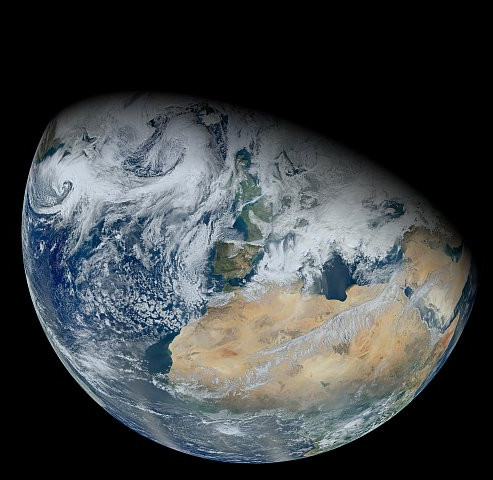
\includegraphics[width=\linewidth]{img/NASA-VIIRS_3Feb2012}
    }
    \column{0.6\textwidth} {
      \begin{itemize}
      \item<1-> \textit{Mathematical} descriptions of general circulation of
        % general circulation of  planetary
        atmosphere and oceans
      \item<2-> Basic components for \textit{climate models}
        \begin{itemize}
        \item Where other equations (e.g. chemical or
          biological) may be coupled
        \end{itemize}
        % \begin{itemize}
        % \item {Weather forecasting, climate understanding, predicting climate evolution...}
        % \end{itemize}
      % \item<3-> Increase of computer power $\Rightarrow$ becoming \textit{more feasible}
       \item<3-> Obtained from simplifications of extremely \textit{complicated
         equations} coming...
         \begin{itemize}
         \item from % different
           conservation laws in physics
           \strip{(momentum, mass, thermodynamics, \\ density, ...)}
         \item on a rotating sphere (the Earth)
         \end{itemize}
      \end{itemize}
      }
  \end{columns}
\end{frame}

\subsection{Quasi-Hydrostatic equations}
%======================================================================

\begin{frame}{The case of (large scale) ocean}
%----------------------------------------------------------------------
  \begin{itemize}\itemsep0.5em
  \item<1> \structure{The ocean:} A slightly compressible fluid
    endowed with Coriolis and buoyancy forces and a set of
    conservation laws from
    Physics
  \item<2-> Simplification of physical laws:\vspace{-1em}
    \begin{columns}
      \column{0.05\linewidth}
      \column{0.41\linewidth}
      \begin{enumerate}\itemsep1.5em
      \item<3-> Boussinesq hypothesis
        \tikz[na] \coordinate(Lboussinesq);
        \hfill
        \tikz[na] \coordinate(Rboussinesq);
      \item<4-> Cartesian coordinates
        \tikz[na] \coordinate(LbetaPlane);
        \hfill
        \tikz[na] \coordinate(RbetaPlane);
      \item<5-> Vertical scaling
        \tikz[na] \coordinate(LverticalScaling);
        \hfill
        \tikz[na] \coordinate(RverticalScaling);
      \end{enumerate}
      \column{0.54\linewidth}
      \begin{overprint}
        \onslide<3>
        \begin{block}{Boussinesq Hypothesis}
          \begin{itemize}
          % \item \textit{Density} does not depart from a \textit{mean reference value},
          %   $\rho_\star>0$.
          \item \alert{\textit{Density}}, $\rho$, can be considered
            \alert{\textit{constant}}, $\rho_\star$.
          \item \alert{\textit{Except}} where it is multiplied by gravity
            acceleration $g$ (\alert{\textit{buoyancy}} terms)
            % Hence density can be replaced by the constant
            % $\rho_\star$ except in
            % \begin{itemize}
            % \item
              % \textit{buoyancy} term
            % \item conservation of \textit{energy equation}
              % {\color{PHDgrayC} (and state equation)}
          \end{itemize}
        \end{block}
        \onslide<4>
        \begin{block}{Cartesian Coordinates}
          \begin{itemize}
          \item A \textit{local projection} of the Earth surface will be
            assumed
          \item \textit{No loss of generality}: spherical coordinates requires
            only the proper handling of some terms
          \end{itemize}
        \end{block}
        \onslide<5>
        \begin{block}{Vertical Scaling of Domain}
          \vspace{-0.5em}
          \begin{itemize}
          \item The \textit{aspect ratio}
            \begin{equation*}
              \framedmath{\displaystyle\varepsilon = \frac{\text{vertical
                    scales}}{\text{horizontal scales}}}~
                \begin{tabular}[t]{l} is \large\textbf{small} \\[-0.2ex]
                  \tiny\it ~ $10^{-3}$, $10^{-4}$\end{tabular}
            \end{equation*}
%            \pause
          \item Dominant terms can be identified in
            \textit{vertical momentum} equation
          \item Numerical point of view: the problem is
            \textit{rescaled}, obtaining...
            \begin{itemize}
            \item \alert{\textbf{Isotropic domain}}
            \item \alert{\textbf{Anisotropic equations}}
            \end{itemize}
          \end{itemize}
        \end{block}
      \end{overprint}
    \end{columns}
  \end{itemize}

  \begin{tikzpicture}[overlay]
%        \draw<2> [thin, red,opacity=.8, fill=red,fill opacity=0.3](stone) circle (4pt);
%        \path<3>[->,>=latex, PHDredA, shorten >=4pt, opacity=.6]
%        (Lboussinesq) edge [out=0, in=130] (Rboussinesq);
        \draw<3>[->, PHDblue, ultra thick, opacity=.8] (Lboussinesq) -- (Rboussinesq);
        \draw<4>[->, PHDblue, ultra thick, opacity=.8] (LbetaPlane) -- (RbetaPlane);
        \draw<5>[->, PHDblue, ultra thick, opacity=.8] (LverticalScaling) -- (RverticalScaling);
\end{tikzpicture}
\end{frame}


\begin{frame}{The adimensional domain}
 \vspace*{0.5em}
 \alert{\textbf{After geometrical scaling}}, we obtain:
   $$
   \domain = \bigl\{ (\xx,z)\in \Rset^{3} \ /\ \xx=(x,y)\in\surface,\
   -D(\xx)< z < 0 \bigr\},
   $$
   where $\surface\subset\Rset^{2}$ is the surface domain and
   $D:\overline\surface \to \Rset_{+}$ a depth function

   \begin{center}
     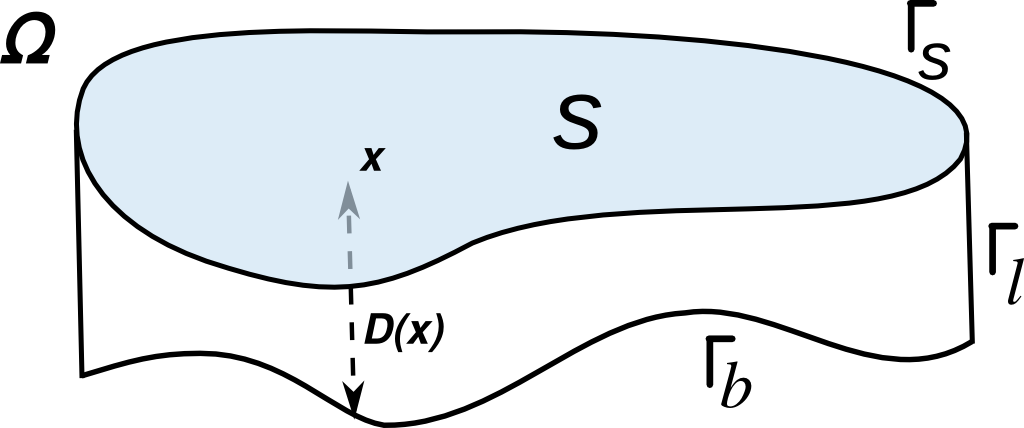
\includegraphics[width=0.66\textwidth]{img/domain}
   \end{center}

   \begin{itemize}
   % \item \alert{Rigid lid hypothesis} (flat surface) is introduced in
   %   this kind of domains
   \item Notation:
     \small
     \llaveizq{      $\surfaceBoundary$: \textbf{surface} boundary
       \\
      $\bottomBoundary$:  \textbf{bottom} boundary
      \\
      $\talusBoundary$: \textbf{lateral walls} (if any)
}
\end{itemize}
 \end{frame}


\begin{frame}{Whole set of Equations}
  %----------------------------------------------------------------------
%  \vspace{-0.2em}
  \note{Comment briefly the main difficulties of Navier--Stokes equations}
  \begin{overprint}
    \onslide<1-2>
    In the adimensional domain:
    \onslide<3>
    \alert{Aspect ratio}:\tikz[na] \coordinate(LaspectRatio);
    \enspace  multiplying vertical velocity terms!
    \onslide<4>
    \alert{\textbf{Coriolis}} force
    \tikz[na] \coordinate(Lcoriolis);
    \onslide<5>
    \alert{\textbf{Buoyancy}} force
    \tikz[na] \coordinate(Lbuoyancy);
    \onslide<6>
    \textbf{Coupling} through \alert{\textbf{density}}~
    \tikz[na] \coordinate(Lcoupling);
  \end{overprint}
  \begin{block}{\small Conservation of momentum and continuity}
    \vspace{-0.66\baselineskip}
    \begin{align*}
      \onslide<1-2>{\text{\tiny Horizontal m.}} &\qquad\enspace \dt \uu + \uu\cdot\gradx\uu + \vv\,\dz\uu  - \visc\Delta\uu
      + \frac 1 \rho_\star \gradx \pp=
       \tikz[na] \node (Rcoriolis) {\framedmath<4>{\fU}};
      \\
      \onslide<1-2>{\text{\tiny Verical m.}} &\quad \tikz[na] \coordinate(RaspectRatio);
        \framedmath<3>{ \alert<3>{\varepsilon^2} \Big( \dt \vv + \uu\cdot\gradx\vv +
          \vv\,\dz\vv - \visc\Delta\vv \Big) }
        \displaystyle
        + \frac 1 \rho_\star \dz \pp
      =
        -\frac{
          \tikz[na] \coordinate(RcouplingA);
          \framedmath<5-6>{\rho}\,\framedmath<5>{\gravity}}{\rho_\star}
         \hskip+0.5em
      \\[-0.1em]
      \onslide<1-2>{\text{\tiny Continuity}} &\qquad\enspace \divx\uu + \dz\vv = 0\hskip+0.5em
    \end{align*}
    \vspace{-1.4\baselineskip}
  \end{block}
  \begin{block}<2->{\small Convection-diffusion of \textit{temperature} and
      \textit{salinity} + state equation (density)}
    \vspace{-0.66\baselineskip}
    \begin{align*}
      \onslide<2>{\text{\tiny Temperature}} &\quad \dt \Te  + (\uu \cdot \gradx) \Te + (\vv\cdot\dz) \Te  - \nu_\Te\Delta \Te = \fT \quad
      \\[0.3em]
      \onslide<2>{\text{\tiny Salinity}} &\quad \dt \Sa  + (\uu \cdot \gradx) \Sa + (\vv\cdot\dz) \Sa -
      \nu_\Sa\Delta \Sa = \fS
      \\[0.3em]
      \onslide<2>{\text{\tiny Density (state eq.)}} &\quad \tikz[na] \coordinate(RcouplingB);
      \framedmath<6>{\rho} = \rho_\star\big(1-\beta_\Te(\Te-\Te_\star) + \beta_\Sa(\Sa-\Sa_\star)\big)
    \end{align*}
    \vspace{-1.4\baselineskip}
  % \item Equation of state (dependence of density in terms of
  %   temperature and salinity)
  %   where $\Te_\star$ and $\Sa_\star$ are given reference values.
  \end{block}
  \tikzstyle{RaspectRatio} = [draw, circle, minimum size=.5cm, node
  distance=1.75cm]
  \tikzstyle{redcircle} = [draw, circle, color=PHDredA, node distance=3cm,
  minimum height=2em]

  \begin{tikzpicture}[overlay]
    \path<3>[myarrow]
    (LaspectRatio) edge [out=320, in=130] (RaspectRatio);
    \path<4>[myarrow]
    (Lcoriolis) edge [out=0, in=130] (Rcoriolis);
    \path<5>[myarrow]
    (Lbuoyancy) edge [out=0, in=130] (RcouplingA);
    \path<6>[myarrow]
    (Lcoupling) edge [out=0, in=135] (RcouplingA);
    \path<6>[myarrow]
    (Lcoupling) edge [out=0, in=135] (RcouplingB);
        % \draw<3>[->, PHDblue, ultra thick, opacity=.8] (Lboussinesq) -- (Rboussinesq);
        % \draw<4>[->, PHDblue, ultra thick, opacity=.8] (LbetaPlane) -- (RbetaPlane);
        % \draw<5>[->, PHDblue, ultra thick, opacity=.8] (LverticalScaling) -- (RverticalScaling);
  \end{tikzpicture}
\end{frame}


\begin{frame}{The case of constant density}
  %----------------------------------------------------------------------
  In the first part of this work, we fix the following usual
  assumption:

  \begin{center}
    \alert{density is a known constant}, e.g. $\rho=\rho_\star>0$
  \end{center}
  \vspace*{0.66em}
  \begin{itemize}\itemsep0.6em
  \item<1-> Then fluid motion equations can be treated independently
  \item<2-> If \tikz[na] \node (LrhoG) {$\rho g$};
    is written as potential... then
    \uncover<3->{it can be absorbed by pressure
      \tikz[na] \coordinate(LpressureAbsorb);}

  \begin{overprint}
    \onslide<1>
    \begin{block}{\small Conservation of momentum and continuity}
      \vspace{-1.3\baselineskip}
      \begin{align*}
        \dt \uu + \uu\cdot\gradx\uu + \vv\,\dz\uu - \visc\Delta\uu +
        \frac 1 \rho_\star \gradx \pp &= \fU
        \\
        \tikz[na] \coordinate(RaspectRatio); \varepsilon^2 \Big( \dt \vv
        + \uu\cdot\gradx\vv + \vv\,\dz\vv - \visc\Delta\vv \Big)
        + \dz \pp
        + \rho\gravity
        &= 0
        \\
        \divx\uu + \dz\vv &= 0
      \end{align*}
      \vspace{-1.4\baselineskip}
    \end{block}
    \onslide<2>
    \begin{block}{\small Conservation of momentum and continuity}
      \vspace{-1.3\baselineskip}
      \begin{align*}
        \dt \uu + \uu\cdot\gradx\uu + \vv\,\dz\uu - \visc\Delta\uu +
        \gradx \pp= \fU
        \\
        \varepsilon^2 \Big( \dt \vv
        + \uu\cdot\gradx\vv + \vv\,\dz\vv - \visc\Delta\vv \Big)
        + \dz \pp +
%        \tikz[na] \coordinate;
        \tikz[na] \node[draw, circle, color=PHDredA, fill
        opacity=1] (RrhoG) {$\rho\gravity$};
        = 0
        \\
        \divx\uu + \dz\vv = 0
      \end{align*}
      \vspace{-1.4\baselineskip}
    \end{block}
    \onslide<3->
    \begin{block}{\small Conservation of momentum and continuity}
      \vspace{-1.3\baselineskip}
      \begin{align*}
        \dt \uu + \uu\cdot\gradx\uu + \vv\,\dz\uu - \visc\Delta\uu +
        \gradx \pp= \fU
        \\
        \framedmath<4>{\varepsilon^2 \Big( \dt \vv + \uu\cdot\gradx\vv + \vv\,\dz\vv -
        \visc\Delta\vv \Big)}
        +
        {\color<3>{PHDred} \tikz[na] \node[draw, circle, fill opacity=1]
        (RpressureAbsorb) {$\dz \pp$};} = 0
        \\
        \divx\uu + \dz\vv = 0
      \end{align*}
      \vspace{-1.4\baselineskip}
    \end{block}
  \end{overprint}
  \vspace{0.66em}
\item<4-> Horizontal / \myframed<4>{vertical} momentum \textbf{anisotropy} \dots
  \end{itemize}

  \begin{tikzpicture}[overlay]
    \path<2>[->,>=latex, PHDredA, shorten >=4pt, opacity=.6, very thick]
    (LrhoG) edge [out=-20, in=120] (RrhoG);
    \path<3>[->,>=latex, PHDredA, shorten >=4pt, opacity=.6, very thick]
    (LpressureAbsorb) edge [out=-45, in=45] (RpressureAbsorb);
  \end{tikzpicture}
 \end{frame}

\begin{frame}{Anisotropic Navier--Stokes equations}
  %----------------------------------------------------------------------
  % \vspace*{0.5em}
  \begin{BlockNoTitle}
    \begin{tabular}{@{}l|>{$}r<{$}>{$}l<{$}@{}}
      \multirow{3}{*}{
        \begin{turn}{30}
          \small\aniNS
        \end{turn}
        }
        &
        \dt \uu + \alert<2>{\uu\cdot\gradx\uu + \vv\,\dz\uu} - \visc\Delta\uu +
        \gradx \pp &= \fU
        \\[0.2em]&
        \varepsilon^2 \Big( \dt \vv + \alert<2>{\uu\cdot\gradx\vv + \vv\,\dz\vv} -
        \visc\Delta\vv \Big)
        + \dz \pp &= 0
        \\[0.2em]&
        \div\uu + \dz\vv &= 0
      \vspace{-1.4\baselineskip}
    \end{tabular}
  \end{BlockNoTitle}

  \medskip
  \uncover<2-> {If $\framedmath<2>{\varepsilon=1}$, we get standard $O(1)$ \alert<2>{Navier--Stokes} equations
  \par  \hfill
  ...but $\varepsilon=1$ is  not realistic in geophysical domains (\exclamation)}
  \vfill
  \medskip

  \uncover<3->{
  Better approaches:}
  \begin{enumerate}\itemsep0.5em
  \item<3-> $\framedmath<3>{0<\varepsilon\lesssim 10^{-3}}$:
    ``\textit{\bfseries\alert<3>{Quasi--Hydrostatic}}'' Navier--Stokes Equations
    \vspace*{0.5em}
    \begin{itemize}
    \item<3-> Realistic model in geophysical domains, e.g.
      $$
      \varepsilon = \frac{\text{5,121 m}}{\text{3,700 km}}
      \quad
      \text{(Mediterranean Sea)}
      $$
    \vspace*{-1.2em}
    \end{itemize}
  \item<4-> \framedmath<4>{\varepsilon=0}: \textbf{\alert<4>{Hydrostatic}} Navier--Stokes or Primitive Equations
  \end{enumerate}
\end{frame}

\begin{frame}{Hydrostatic Navier--Stokes (or Primitive) equations}
%------------------------------------------------------------
  In practice, the simplification \framedmath{\varepsilon=0} is usually taken,
  obtaining:
\begin{block}{}
  \begin{tabular}{@{}l|>{$}r<{$}>{$}l<{$}@{}}
    \multirow{3}{*}{
      \begin{turn}{30}
        \small \hydNS
      \end{turn}
    }
    &
    \dt\uu + (\uu\cdot\gradx)\uu +\vv\dz \uu
    - \visc\Delta\uu + \gradx\pp &= \ff \ \In\domain,
    \label{eq:HNS.a}
    \\
    &
    \dz\pp & = 0 \ \In\domain,
    \label{eq:HNS.b}
    \\
    &
    \divx\uu +  \dz\vv &= 0 \ \In\domain.
    \label{eq:HNS.c}
  \end{tabular}
\end{block}
\begin{itemize}
\item Originally derived from scale analysis~\cita{Pedlosky:1987,CushmanRoisin-Beckers:09}
\item Mathematically justified as limit of anisotropic Navier--Stokes \aniNS,
  when $\varepsilon\to 0$ in vertical momentum
  equation~\cita{Besson-Laydi:92,Azerad-Guillen:01}
% \item Complemented with adequate boundary
%   conditions.
% ~(\ref{eq:bc.1})--(\ref{eq:bc.3}). See that, now,
%   it is natural not imposing boundary conditions for $\vv$ on
%   $\talusBoundary$.
\end{itemize}
\end{frame}

% \begin{frame}{Vertical integration of Hydrostatic Navier--Stokes}
%   \begin{itemize}
%   \item Model widely studied (both theoretically and in numerical
%     simulations)
%   \item Almost all works use the following \emph{\structure{vertical integrated formulation
%           of the primitive equations}}: find $\uu:\domain\times (0,T)
%       \to \Rset^2$, horizontal velocity, and $\ps:\domain\times (0,T)
%       \to\Rset$, (artificial) surface pressure, such that
%       \begin{BlockNoTitle}
%         \begin{tabular}{@{}l|>{$}r<{$}>{$}l<{$}@{}}
%           \multirow{3}{*}{
%             \begin{turn}{30}
%               \small\reducedProblem
%             \end{turn}
%           }
%           &
%           \dt\uu + (\uu\cdot\gradx)\uu +\vv\dz \uu - \visc\Delta\uu +
%           \gradx\ps = \ff & \In\domain,
%           \label{eq:EP.a}
%           \\
%           &
%           \divx\langle\uu\rangle = 0 & \In\domain,
%           \label{eq:EP.b}
%           \\
%           &
%           \uu = 0 \quad \On\bottomBoundary\cup\talusBoundary, \qquad
%           \visc_z\dz\uu = \gs &\On \surfaceBoundary,
%           \label{eq:EP.c}
%         \end{tabular}
%       \end{BlockNoTitle}
%       where $\vv$ and $\langle\uu\rangle$ are defined by:
%   $$
%   \vv(\xx,\zz,t) = \int_z^0 \divx\uu(\xx,s,t)\;ds, \qquad
%   \langle\uu\rangle(\xx,t) = \int_{-D(\xx)}^0 \uu(\xx,\zz,t) dz.
%   $$
%       \begin{itemize}
%     \item Integrate in $z$ the divergence equations in ~\hydNS
%     \item Use account the rigid lid hypothesis~(\ref{eq:bc.2})
%     \end{itemize}
%     we obtain the
%       next equivalent
% \end{itemize}
% \end{itemize}
% \end{frame}

\begin{frame}{Vertical integration of Hydrostatic Navier--Stokes}
  \begin{itemize}\itemsep0.77ex
  \item Widely studied \soften{(both theoretically and in numerical
    simulations)}
  \item Almost all works \soften{use the following equivalent}
    \textbf{\alert{vertical integrated formulation of the primitive
        equations}}:
    \begin{itemize}
    \item find $\uu:\domain\times (0,T) \to \Rset^2$ (horizontal
      velocity) and
    \item $\ps:\surface\times (0,T) \to\Rset$ (artificial surface
      pressure) such that
    \end{itemize}
    \begin{BlockNoTitle}
      \begin{tabular}{@{}l|>{$}r<{$}>{$}l<{$}@{}}
        \multirow{3}{*}{
          \begin{turn}{30}
            \small\reducedProblem
          \end{turn}
        }
        &
        \dt\uu + (\uu\cdot\gradx)\uu +\vv\dz \uu - \visc\Delta\uu +
        \gradx\ps = \ff & \In\domain,
        \label{eq:EP.a}
        \\
        &
        \divx\langle\uu\rangle = 0 & \In\domain,
        \label{eq:EP.b}
        \\
        &
        \uu = 0 \quad \On\bottomBoundary\cup\talusBoundary, \qquad
        \visc_z\dz\uu = \gs &\On \surfaceBoundary,
        \label{eq:EP.c}
      \end{tabular}
    \end{BlockNoTitle}
    where $\vv$ and $\langle\uu\rangle$ are defined by:
    \vspace{-0.5em}
    $$
    \vv(\xx,\zz,t) = \int_z^0 \divx\uu(\xx,s,t)\;ds, \qquad
    \langle\uu\rangle(\xx,t) = \int_{-D(\xx)}^0 \uu(\xx,\zz,t) dz.
    $$
  \item It is obtained...
    \begin{itemize}
    \item Integrating in $z$ the divergence equations in ~\hydNS
    \item Using the \textbf{rigid lid hypothesis}
    \end{itemize}
  \end{itemize}
\end{frame}

\begin{frame}
\frametitle{Comparison of the models}
\vspace{0.5em}
\small
\begin{tabularx}{\textwidth}{@{}X@{\qquad}X@{}}
  {\bf Integrated model \reducedProblem} &
  {\bf Not integrated \aniNS}
  \\ \toprule
  System of \textit{3 PDE} + 3 unknowns: \ \good&
  System of  \textit{4 PDE} +   4 unknowns: \ \bad
  \\ %\midrule
    % 3 unknowns\ \good\ :
    \hspace{17ex}
    \begin{tabular}[b]{l}
      $\uu$ (in $\domain$) \\ $\ps$ (in $\surface$) \ \good
    \end{tabular}
    &
  % 4 unknowns \bad \ :
      \hspace{17ex}
      \begin{tabular}[l]{l}
      $\uu$ (in $\domain$), \\  $\vv$ (in $\domain$),
      \\ $\pp$ (in $\domain$) \ \bad
    \end{tabular}
    % $\vv=\vv(\uu)$
    \\ \midrule
    $\vv=\vv(\uu)$ is \emph{decoupled} \ \good
    &
    $\vv$ is \textit{not decoupled}\ \bad
  \\ \midrule
   Differential
  $+$ z-\emph{integral} pb. \ \bad
  &
  Only differential problems \ \good
  \\ \midrule
  Structured meshes\ \bad
  &
  Unstructured or struct. meshes \ \good
  \\
  % \begin{center}\vspace{-2em}
  \hspace{-3.2ex}
    \hfill\pgfimage[width=3.5cm]{img/struct-mesh}\hfill\qquad~
  % \end{center}
%  \\ \bottomrule
    &
  % \begin{center}\vspace{-2em}
  \hspace{-3.2ex}
    \hfill\pgfimage[width=3.5cm]{img/unstruct-mesh}\hfill\qquad~
  % \end{center}
    \\ \hline
    Needs simplification $\varepsilon=0$\ \bad
    &
    More general models, $\varepsilon\ge 0$\ \good
  \\ \midrule
  {\scriptsize Less flexibility for include extensions} \bad
  &
  {\scriptsize Flexibility (extensions like mesh adaptivity)}\good
\end{tabularx}
\end{frame}

% \begin{frame}
% \frametitle{Comparison of the models}
% \vspace{0.5em}
% \small
% \begin{tabularx}{\textwidth}{@{}X@{\qquad}X@{}}
%   {\bf Not integrated \aniNS}  & {\bf Integrated model \reducedProblem}
%   \\ \toprule
%   System of  4 PDE +   4 unknowns: \ \bad &
%   System of 3 PDE + 3 unknowns: \ \good
%   \\ %\midrule
%   % 4 unknowns \bad \ :
%       \hspace{17ex}
%       \begin{tabular}[l]{l}
%       $\uu$ (in $\domain$), \\  $\vv$ (in $\domain$),
%       \\ $\pp$ (in $\domain$) \ \bad
%     \end{tabular}
%     % $\vv=\vv(\uu)$
%     &
%     % 3 unknowns\ \good\ :
%     \hspace{17ex}
%     \begin{tabular}[b]{l}
%       $\uu$ (in $\domain$) \\ $\ps$ (in $\surface$) \ \good
%     \end{tabular}
%     \\ \midrule
%     $\vv$ is not decoupled\ \bad
%     &
%     $\vv=\vv(\uu)$ is decoupled \ \good
%   \\ \midrule
%   Only differential problems \ \good  &  Differential
%   $+$ z-integral pb. \ \bad
%   \\ \midrule
%   Unstructured or struct. meshes \ \good &
%   Structured meshes\ \bad
%   \\
%   % \begin{center}\vspace{-2em}
%   \hspace{-3.2ex}
%     \pgfimage[width=3.5cm]{img/unstruct-mesh}
%   % \end{center}
%   &
%   % \begin{center}\vspace{-2em}
%   \hspace{-3.2ex}
%     \pgfimage[width=3.5cm]{img/struct-mesh}
%   % \end{center}
% %  \\ \bottomrule
%     \\ \hline
%     More general models, $\varepsilon\ge 0$\ \good &
%     Needs simplification $\varepsilon=0$\ \bad
%   \\ \midrule
%   {\scriptsize Flexibility (extensions like mesh adaptivity)}\good &
%   {\scriptsize Less flexibility for include extensions} \bad
% \end{tabularx}
% \end{frame}

\begin{frame}{Our objectives}
\begin{enumerate}\itemsep0.66em
\item \textit{Analysis} of the pecularities (the stability) of
  Navier--Stokes in geophysical domains (where $\varepsilon$ is ``small'')
\item Use this analysis to \textit{propose some new FE
    combinations} which:% fulfill the following \textit{purposes}:
  \begin{enumerate}\itemsep0.33em
  \item Allow numerically solving \textit{more realistic models than pure hydrostatic
      ones}. Moreover, to achieve solving both Hydrostatic and not
    Hydrostatic Navier--Stokes equations in the same way.
  \item \textit{Avoid the introduction of integro-differential equations},
    exploiting the advantages of non-integral models (enounced above)
  \end{enumerate}
\item Develop \textit{new discrete schemes} which are
  stable, when $\varepsilon\to 0$, for usual LBB FE combinations for
  Navier--Stokes (including $\varepsilon=0$)
\item Extend these new schemes to \textit{more complex time-dependent
    problems} (including variable density) and define \textit{new
  time-splitting schemes}
\end{enumerate}
\end{frame}


%%% Local Variables:
%%% coding: utf-8
%%% TeX-master: "JRRG-pde-ocean"
%%% mode: latex
%%% ispell-local-dictionary: "english"
%%% End:



%%,---------------------------------------------------------------------
%%| Conclusions and future work
%%`---------------------------------------------------------------------
\begin{frame}{Conclusions}
  \begin{itemize}\itemsep0.66em
  \item<1-> We have developed \alert{new schemes} for approximation of
    Primitive Equations of the Ocean (or even Anisotropic Navier-Stokes)
    \begin{itemize}
    \item Avoiding velocity instabilities of (quasi-)hydrostatic
      formulations
    \end{itemize}
  \item<2-> \alert{Standard FE tools and techniques} like mesh adaptation
    can be used, in \alert{more general meshes} than previous schemes
  \item<3-> Two different approached have been followed:
    \begin{itemize}
    \item New \alert{stable combinations of FE} (unequal
      approximation of velocity components)
    \item Reformulation of space schemes, \alert{stabilizing vertical
      velocity}. Hence standard Stokes--stable FE can be applied
    \end{itemize}
  \item<4-> Successfully applied to \alert{time-dependent problems},
    including \alert{variable density}
  \end{itemize}
  \uncover<5>{
  \begin{center}\it
    {In short, we have successfully introduced \textbf{a new approach}\\
    for modelling \textbf{realistic hydrostatic and quasi-hydrostatic fluids},\\
    justifying it both \textbf{analytically and numerically}.
  }
\end{center}
}

\end{frame}
\begin{frame}{~}
  \bigskip
  \Large Thank you for your attention.
  \vfill~
  \begin{flushright}
    \pgfsetfillopacity{0.4}
    \pgfimage[width=0.9\textwidth]{img/gibraltar-velocity-2d-difumin}
  \end{flushright}
\end{frame}

%%,-------------
%%| Bibliography
%%`-------------

\setbeamertemplate{footline}[default]

\begin{frame}[allowframebreaks]{Bibliography}
\bibliographystyle{alpha}
%\bibliographystyle{abbrvnat}
\bibliography{biblio-short.bib}
\end{frame}

\end{document}


%%% Local Variables:
%%% coding: utf-8
%%% TeX-master: t
%%% mode: latex
%%% ispell-local-dictionary: "english"
%%% End:
